\documentclass{article}

\usepackage[version=3]{mhchem} % Package for chemical equation typesetting
\usepackage{siunitx} % Provides the \SI{}{} and \si{} command for typesetting SI units
\usepackage{graphicx} % Required for the inclusion of images
\usepackage{natbib} % Required to change bibliography style to APA
\usepackage{amsmath} % Required for some math elements 
\usepackage[labelformat=empty]{caption}
\usepackage{enumitem}

\setlength\parindent{0pt} % Removes all indentation from paragraphs

\renewcommand{\labelenumi}{\alph{enumi}.} % Make numbering in the enumerate environment by letter rather than number (e.g. section 6)

%\usepackage{times} % Uncomment to use the Times New Roman font

%----------------------------------------------------------------------------------------
%	DOCUMENT INFORMATION
%----------------------------------------------------------------------------------------

\title{Algorytmy i Struktury Danych II \\ ZESTAW 02} % Title

\author{} % Author name

\date{} % Date for the report

\begin{document}

\maketitle % Insert the title, author and date

\begin{center}
\begin{tabular}{l r}
%Data labolatorium: & 29.03.2022 \\
Autor: & Marcin \textsc{Wolski}
\end{tabular}
\end{center}

\section*{Typ danych setHashed}

Typ danych setHashed reprezentuje matematyczny zbiór oraz operacje które dla dwóch zbiorów realizują: 
\begin{itemize} 
    \item sumę zbiorów
    \item część wspólną zbiorów
    \item różnicę zbiorów
    \item sprawdzanie identyczności zbiorów
\end{itemize}
oraz dla elementu zbioru realizują: 
\begin{itemize}
    \item wstawanie elementu do zbioru
    \item usuwanie elementu ze zbioru
    \item sprawdzanie czy element należy do zbioru
\end{itemize}
Wykorzystuje hashowanie otwarte. 

\subsection*{Badanie złożoności operacji}
 Czas wykonania operacji zmierzony został dla zbiorów o rozmiarach [1, 500]. Dla każdej wielkości obliczona została średnia z 1000 powtórzeń działania. Wygenerowane zostały pliki z danymi które zwizualizowane zostały za pomocą programu gnuplot.
\subsection*{Wykresy}

\begin{center}
    \textit{Wstawianie elementu\\}
    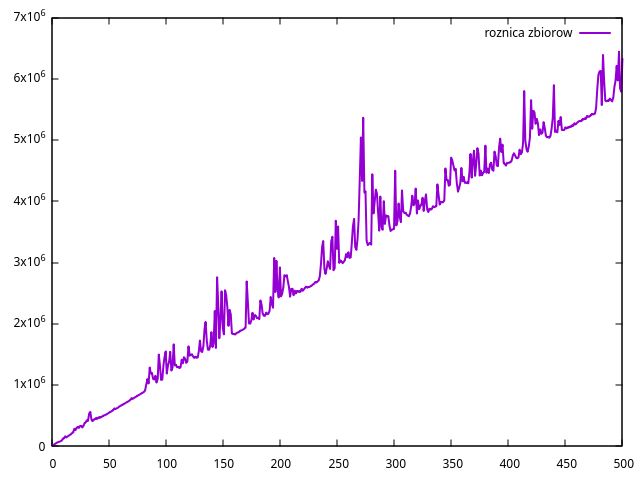
\includegraphics[width=0.7\textwidth]{difference}\\
    \textit{Przecięcie dwóch zbiorów\\}
    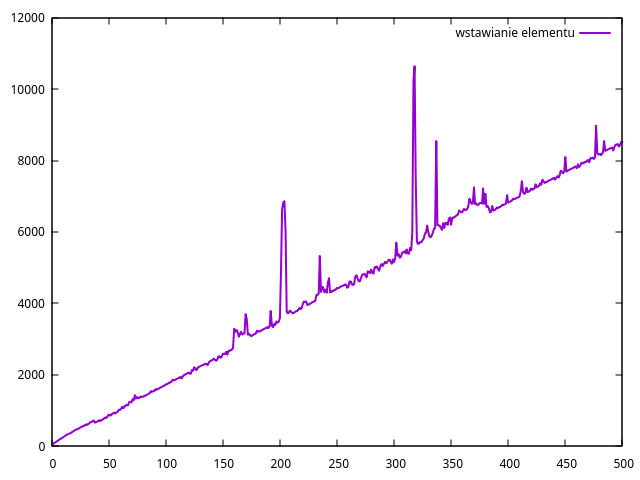
\includegraphics[width=0.7\textwidth]{insert}\\
    \textit{Suma dwóch zbiorów\\}
    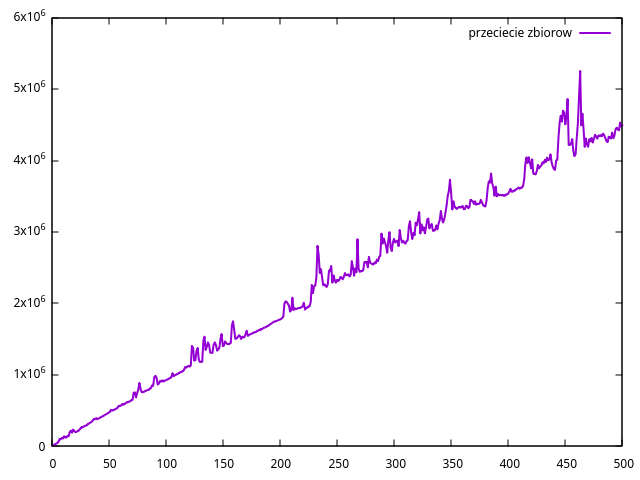
\includegraphics[width=0.7\textwidth]{intersection}\\
    \textit{Suma dwóch zbiorów\\}
    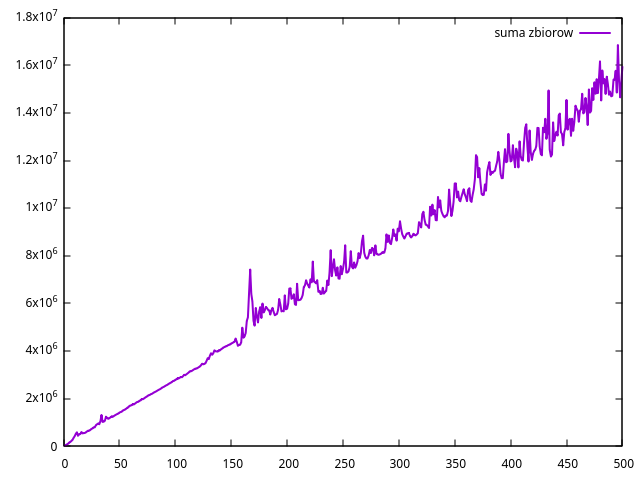
\includegraphics[width=0.7\textwidth]{unify}\\
\end{center}

\cite{}
\end{document}